\documentclass[12pt,a4paper]{article}
 \usepackage[italian]{babel}
 \usepackage[latin1]{inputenc}
 \usepackage{verbatim}
 \usepackage{amsmath}
 \usepackage{graphicx}
 \usepackage{url}
 \usepackage{geometry}
 \usepackage{color}
 \usepackage{subfigure}
 \usepackage{multirow}
 \newenvironment{sistema}%
  {\left\lbrace\begin{array}{@{}l@{}}}%
  {\end{array}\right.}
 
 \geometry{a4paper,top=3cm,bottom=3cm,left=1.5cm,right=1.5cm,heightrounded,bindingoffset=1cm}
 
 \begin{document}
 	\title{Modello matematico con tre masse e tre molle smorzate} \author{Matteo Bolognese}
 	\date{23/11/2019}
 	\maketitle
 	
 \section{Introduzione}
	La misura sperimentale della costante elastica dinamica di un materiale $K(\omega)$ per mezzo di un martello strumentato \'e stata effettuata con diverse configurazioni di misura. Una delle pi\'u semplici, rappresentata in \figurename~\ref{fig:Phisical-configuration}, prevede il posizionamento di una piastra di carico sul campione a sua volta poggiato al suolo. La piastra di carico vuiene colpita con il martello strumentato e uno o pi\'u accelerometri misurano l'accelerazione della piastra e/o del suolo a seconda degli intenti della misura.
	Al duplice scopo di validare le misure sperimentali e di estrapolare correttamente i valori di costate elastica dinamica del campione dai grafici sperimentali \'e utile sviluppare un modello matematico che riproduca il comportamento del sistema.
	
	\begin{figure}
		\centering
		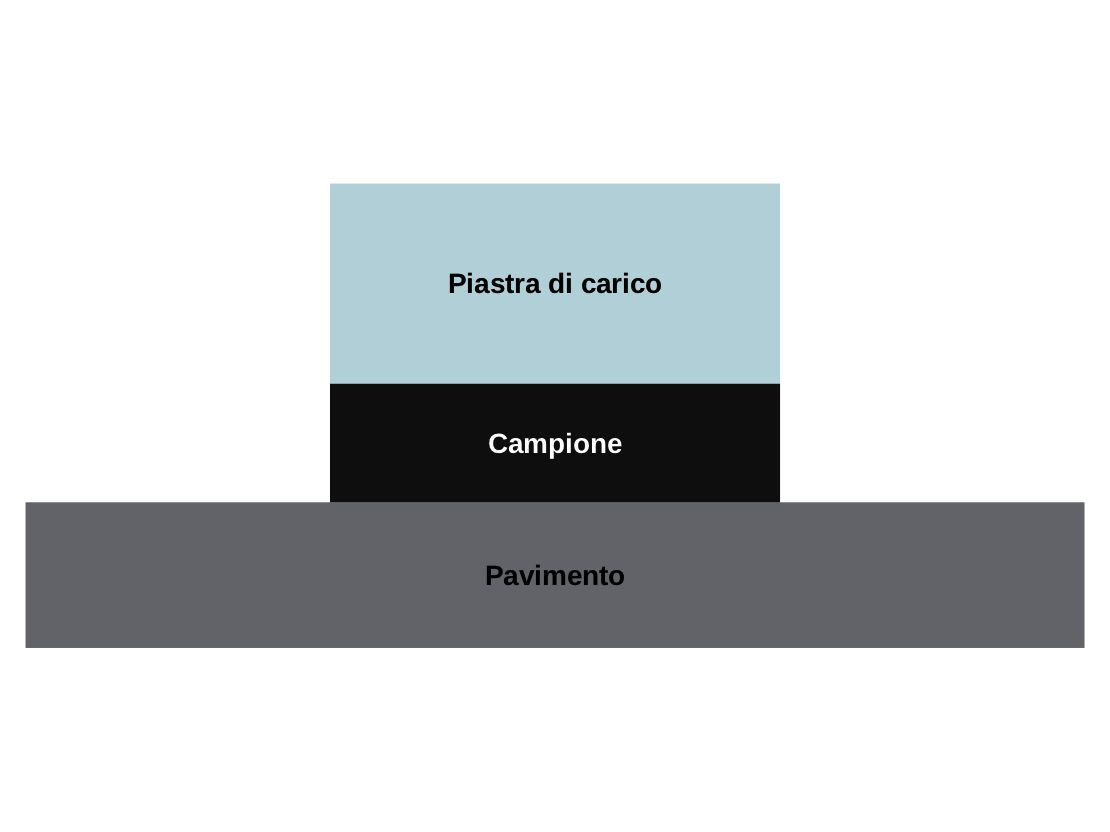
\includegraphics[width=8cm]{Phisical-system.jpg}
		\caption{Configurazione sperimentale.}
		\label{fig:Phisical-configuration}
	\end{figure}
 	
 \section{Tre masse e tre molle smorzate}
 	La pi\'u semplice rappresentazione matematica che conservi un sufficiente livello di dettaglio per rappresentare correttamente quanto misurato sperimentalmente \'e riportata in \figurename~\ref{fig:model} e consiste in un sistema di tre masse e tre oscillatori smorzati. Gli indici 1, 2 e 3 sono riferiti rispettivamente alla piastra, al campione e al solaio. Facciamo notare come la coordinata x \'e orientata dal basso verso l'alto quindi concorde con la direzione di misura degli accelerometri, ma discorde al verso del martello strumentato, che misura positiva una forza diretta dall'alto verso il basso. In fase di elaborazione delle misure sar\'a quindi necessario introdurre un cambio di segno nella forza o nelle accelerazioni.
 	Le coordinate generalizzate x\ped{i} rappresentano le distanze delle tre masse dalle posizioni di equilibrio x\ped{i,0}.
 	\begin{figure}
 		\centering
 		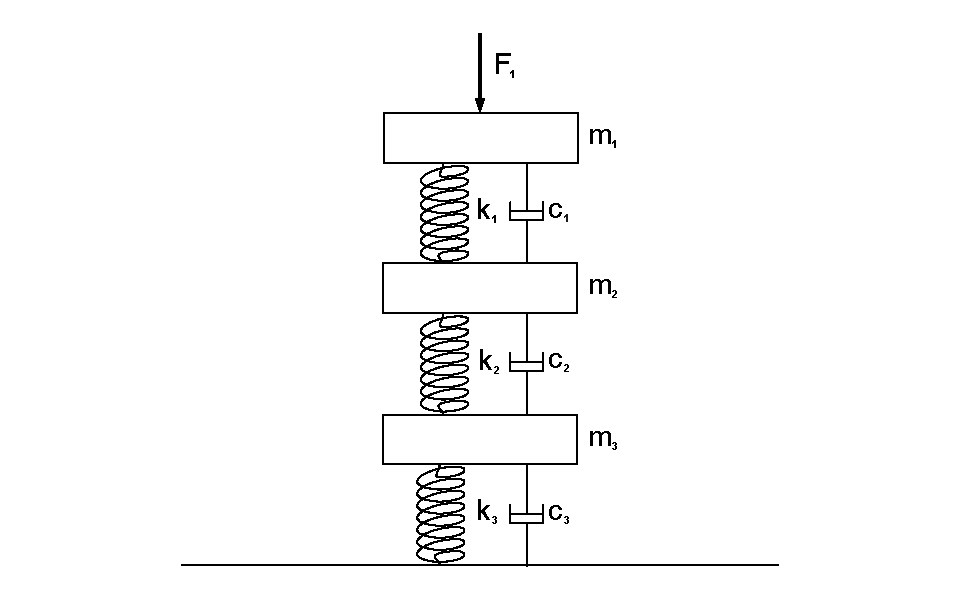
\includegraphics[width=10cm]{model}
 		\caption{Modello teorico.}
 		\label{fig:model}
 	\end{figure}
 	
 	
 	\subsection[Lagrangiana]{Trattazione lagrangiana}
 		Un metodo efficace di ricavare le equazioni del moto di un sistema dinamico \'e quello lagrangiano (introdurre citazione) che si basa sulla determinazione di due quantit\'a fondamentali, l'energia meccanica totale $T$ e dell'energia potenziale $V$ del sistema. Nel nostro caso l'energia meccanica totale non \'e altro che la somma delle energie cinetiche delle tre masse:
 		\begin{equation}
 			T= \frac{1}{2} m_1 \dot x_1^2 +\frac{1}{2} m_2 \dot x_2^2+ \frac{1}{2}m_3 \dot x_3^2 
 			\label{eq:mechanical-energy}
 		\end{equation}
 		dove $\dot x_i$ \'e la velocit\'a della massa $i$-esima.
 		L'energia potenziale \'e invece la somma delle energie potenziali delle molle:
 		\begin{equation}
 			V= \frac{1}{2} k_1(x_1-x_2)^2+\frac{1}{2} k_2(x_3-x_2)^2 + \frac{1}{2} k_3 x_3^2
 			\label{eq:potential-energy}
 		\end{equation}
 		I contributi dovuti all'azione degli smorzatori verranno invece introdotti successivamente con la veste di forze esterne in quanto estranee all'azione delle molle.
 		A questo punto le equazioni differenziali si ottengono attraverso la seguente eguaglianza: 		
 		\begin{equation}
 			\frac{d}{dt} \frac{\partial T}{\partial \dot x_i} - \frac{\partial T}{\partial x_i} + \frac{\partial V}{\partial x_i}=F_i
 			\label{eq:lagrangian}
 		\end{equation}
 		dove $F\ped{i}$ \'e la risultante della forze esterne e delle forze dissipative agenti sull'$i$-esima massa. Siccome l'energia meccaneca del sistema non dipende dalle $x\ped{i}$ il secondo termine dell'equazione (\ref{eq:lagrangian}) \'e automaticamente nullo. Deriviamo dunque l'energia meccanica rispetto alle velocità $\dot x\ped{i}$ e quindi rispetto al tempo:
 		\begin{equation}
 			\frac{d}{dt} \frac{\partial T}{\partial \dot x_i}= \frac{d}{dt} m_i \dot{x}_i =m_i \ddot{x}_i
 			\label{eq:energie}
 		\end{equation}
 		
		La derivata parziale di V rispetto alle coordinate generalizzate produce invece:
		
		\begin{gather}
 		\begin{cases}
 		\frac{\partial V}{\partial x_1}= k_1(x_1 - x_2)
 		\\
 		\frac{\partial V}{\partial x_2} = - k_1(x_1 - x_2) - k_2(x_3 - x_2)
 		\\
 		\frac{\partial V}{\partial x_3} = (k_3 +k_2)x_3-k_2 x_2
 		\label{eq:potenziali}
		\end{cases}
		\end{gather}
		
 		Combinando le equazioni \ref{eq:energie} e \ref{eq:potenziali} otteniamo il sistema:
		
		\begin{gather}
 		\begin{sistema}
 			m_1 \ddot{x}_1 + k_1x_1 - k_1 x_2 = F_1
 			\\
 			m_2 \ddot{x}_2 - k_1 x_1 + (k_1 +k_2 )x_2 - k_2 x_3  = F_2
 			\\
 			m_3 \ddot{x}_3 + (k_3+k_2) x_3 -k_2 x_2= F_3
 			\label{eq:sistema-1}
 		\end{sistema}
		\end{gather}
 		
		Resta da identificare le forze dissipative $F_{ d,i}$ agenti sulle tre masse, definite come segue:
 		
		\begin{equation}
 			F_{ d,i} = - \sum_{\substack{k}} c_{ik} \dot{x}_k
 		\end{equation}
 		dove c\ped{ik} \'e la forza agente sulla $i$-esima massa quando la massa $k$-esima si muove con velocit\'a unitaria, per cui otteniamo:
		\begin{gather}
 		\begin{cases}
		c_{11} = c_{1}
		\\
		c_{22} = c_{1} + c_{2}
		\\
		c_{33} = c_{2} + c_{3}
		\\
		c_{12} = c_{21} = - c_{1}
		\\
		c_{23} = c_{32} = - c_{2}
		\\
		c_{13} = c_{31} = 0
		\end{cases}
		\end{gather}
		A questo punto esplicitiamo le forze dissipative:
		\begin{gather}
		\begin {sistema}
		F_{d1} = - c_{11}\dot x_1 - c_{12}\dot x_2 = -c_1 \dot x_1 + c_1 \dot x_2
		\\
		F_{d2} = - c_{21}\dot x_1 - c_{22}\dot x_2 - c_{23}\dot x_3 = c_1  \dot x_1  - (c_1 + c_2) \dot x_2 + c_2\dot x_3
		\\
		F_{d3} = - c_{32}\dot x_2 - c_{33}\dot x_3 = c_2 \dot x_2 - (c_2 + c_3) \dot x_3		
		\end{sistema}
		\end{gather}
 		ed otteniamo le equazioni complete aggiungendo la forza esterna F\ped 1:
		\begin{gather}
		\begin {sistema}
		m_1 \ddot{x}_1 + k_1x_1 - k_1 x_2  =  -c_1 \dot x_1 + c_1 \dot x_2 +F_1
		\\
		m_2 \ddot{x}_2 - k_1 x_1 + (k_1 +k_2 )x_2 - k_2 x_3 = c_1  \dot x_1  - (c_1 + c_2) \dot x_2 + c_2\dot x_3
		\\
		m_3 \ddot{x}_3 + (k_3 +k_2 )x_3 -k_2 x_2= c_2 \dot x_2 - (c_2 + c_3) \dot x_3
		\end{sistema}
				\label{eq:completa}
		\end{gather}
		
%		Risulta utile riscrivere il sistema nella rappresentazione matriciale che permette una lettura pi\'u comoda e mette in evidenza le propriet\'a di simmetria del sistema.
%		\begin {gather}
%		\begin{vmatrix}
%		m_1 \ddot{x}_1 + k_1x_1	+ c_1 \dot x_1	&  		- k_1 x_2	- c_1 \dot x_2 		&	0 \\
%		- k_1 x_1 - c_1  \dot x_1 				&  	m_2 \ddot{x}_2	+ (k_1 +k_2 )x_2 +(c_1 + c_2) \dot x_2	&	- k_2 x_3 - c_2\dot x_3 \\
%		0	&  	-k_2 x_2 - c_2 \dot x_2		&m_3 \ddot{x}_3 + (k_3 +k_2 )x_3 +(c_2 + c_3) \dot x_3	 \\
%		\end{vmatrix}
%		=
%		\begin{vmatrix}
%		F_1
%		\\
%		0
%		\\
%		0
%		\label{eq:matrix}
%		\end{vmatrix}
%		\end{gather}
	
		A ragione del fatto che la misura sperimentale dell'accelerazione viene effettuata sulla massa m\ped1 ci interessa risolvere il sistema in funzione della coordinata $x\ped{1}$. A tal proposito ipotizziamo che il sistema venga sottoposto a una forza esterna $F(t)$. In generale se la forza $F(t)$ appartiene a  $L^2$ pu\'o essere espressa in funzione di una base dello spazio $L^2(R)$, ad esempio $e^{i\omega t}$ (con $\omega$ positivo e reale) e quindi usare la sua trasformata di Fourier $F(\omega)$. Se l'azione di $F(\omega)$ \'e abbastanza duratura nel tempo in modo da superare la fase transiente il sistema, anche le coordinate generalizzate $x\ped{i} $ seguiranno un andamento del tipo $x\ped{i}(\omega, t)=A\ped{i}(\omega)e^{i\omega t}$. Calcoliamo quindi le derivate prima e seconda di una $x\ped{1}$:
		\begin {gather}
		\begin{sistema}
		\frac{\partial x_i}{\partial t }= i \omega A\ped{i}(\omega)e^{i\omega t}=i \omega x_i
		\\
		\\
		\frac{\partial \dot x_i}{\partial t }= - \omega ^2 A\ped{i}(\omega)e^{i\omega t}=-\omega^2 x_i
		\end{sistema}
		\end{gather}
		
		e sostituiamo nella (\ref{eq:completa}) tenendo implicite le coordinate:
		
		\begin {gather}
		\begin{cases}
		(-m_1 \omega^2  + k_1 + c_1 i\omega)x_1 - (k_1 + c_1 i\omega)x_2& =  F_1 \\
		-(k_1  + c_1  i\omega)x_1 +(-m_2 \omega^2 + (k_1 +k_2 ) + (c_1 + c_2) i\omega)x_2 - (k_2  + c_2 i\omega)x_3& = 0\\
		-(k_2  + c_2 i\omega)x_2+ (-m_3 \omega^2 + (k_3 +k_2) +(c_2 + c_3) i\omega)x_3& = 0\\
		\end{cases}
		\end {gather}
		
		Passando alla rappresentazione matriciale possiamo scrivere:
		
		\begin {gather}
		\begin{vmatrix}
			-m_1 \omega^2  + k_1 	+ c_1 i\omega 	&  	- k_1 	- c_1 i\omega  						&	0\\
			- k_1  - c_1  i\omega  	&  -m_2 \omega^2 	+ (k_1 +k_2 ) +(c_1 + c_2) i\omega 	&	- k_2  - c_2 i\omega \\
			0													&  	-k_2  - c_2 i\omega 	&-m_3 \omega^2 + (k_3 +k_2) +(c_2 + c_3) i\omega
		\end{vmatrix}
		\begin{vmatrix}
		x_1 \\ x_2 \\ x_3
		\end{vmatrix}
		=
		\begin{vmatrix}
			F_1
			\\
			0
			\\
			0
			\label{eq:matrix2}
		\end{vmatrix}
		\end{gather}		
		Dalla terza riga della (\ref{eq:matrix2}) ricaviamo $x_3$ in funzione di $x_2$:
		\begin{equation}
		x_3=x_2 \frac{	+k_2  + c_2 i\omega}{-m_3 \omega^2 + (k_3 +k_2) +(c_2 + c_3) i\omega}  = x_2 A
		\end{equation}
		e riscriviamo la seconda riga:
		\begin{equation*}
		(- k_1  - c_1  i\omega )x_1 	+  \left [- m_2 \omega^2 + (k_1 + k_2) + (c_1 + c_2) i\omega - ( k_2  + c_2 i\omega)A \right] x_2 =0
		\end{equation*}
		\begin{equation}
		x_2=x_1 \frac{+ k_1  + c_1  i\omega}{- m_2 \omega^2 + (k_1 + k_2) + (c_1 + c_2) i\omega + (- k_2  - c_2 i\omega)A} =x_1 B
		\end{equation}
 		e quindi dalla prima riga:
 		\begin{equation*}
		\left[ -m_1 \omega^2  + k_1 	+ c_1 i\omega -( k_1+ c_1 i\omega)B \right]x_1=F_1
 		\end{equation*}
 		\begin{equation*}
 		K_1 (\omega)=\frac{F_1}{x_1 (\omega)}=-m_1 \omega^2  + k_1 + c_1 i\omega -( k_1 + c_1 i\omega)B
		\end{equation*}
		dove $K_1 (\omega)$ \'e la costante elastica dinamica misurata sulla massa $m_1$.
		Ricordando che derivare $x$ nel tempo equivale a moltiplicare per $i \omega$ otteniamo la tra $F_1$ e $\ddot x_1$ otteniamo l'espressione algebrica della Massa Dinamica $M(\omega)$ del sistema la quale verrà utilizzata per generare segnali di test per lo script di elaborazione:
 		\begin{equation}
 		M=\frac{F_1}{\ddot x_1}=\frac{-m_1 \omega^2  + k_1 + c_1 i\omega -( k_1 + c_1 i\omega)B}{-\omega^2}
 		\end{equation}
\section{Dati disponibili}
	Riportiamo in Tabella~\ref{tab:material}  i dati disponibili sui materiali utilizzati e le $k$ statiche attese.
	

	
	


\begin{table}[]
	\centering
	\caption{Propriet\'a meccaniche dei materiali utilizzati}
	\label{tab:material}
	\begin{tabular}{cccccc}
		\hline\hline
		\multirow{2}{*}{Materiale} & Spessore&Superficie&Modulo E & K&Peso\\
		&[m]& [$m^2$]& [GPa]&[GN/m]& [Kg]\\
		\hline
		Piastra pesante 1&$0.024$	& $\pi* 0.05^2=0.0079$	& 180	& 59.3	& 1.4293	\\
		Piastra pesante 2&$0.0475$	& $\pi* 0.05^2=0.0079$	& 180	& 30.0	& 2.8871	\\
		Blocco cemento	&$0.13 $	& $0.25^2=0.0625$		& 45 	& 21.6	& $\sim$ 15	\\
		Polipropilene	&$0.005$	& $0.096*0.098=0.0094$	& 1.5	&  2.8	& 0.0383	\\
		\hline\hline
	\end{tabular}
\end{table}



 \section{Analisi dei segnali}
 I segnali acquisiti sperimentalmente necessitano di essere opportunamente processati per ottenere la risposta in frequenza del sistema.
 \subsection{Ricerca picchi e costruzione matrici dei dati}
 
 \subsection{Filtraggio}
 L'operazione di filtraggio viene effettuata sulla matrice $F$ allo scopo di abbattere il segnale prodotto dal martello dopo il suo distacco dalla superficie del campione e quindi non correlato con l'accelerazione misura sul campione. In \figurename~\ref{fig:Effettofiltraggio} è possibile osservare come l'effetto del filtraggio (operato tramite media mobile) sulla Power Spectral Density si concentri al di sopra della regione in cui lo spettro della Forza risulta piatto e della frequenza di coerenza. Considerando che la stima delle grandezze oggetto della misura avviene al di sotto della frequenza di coerenza, l'operazione di filtraggio  appare in ultima analisi ininfluente.
 \begin{figure}
	\centering
	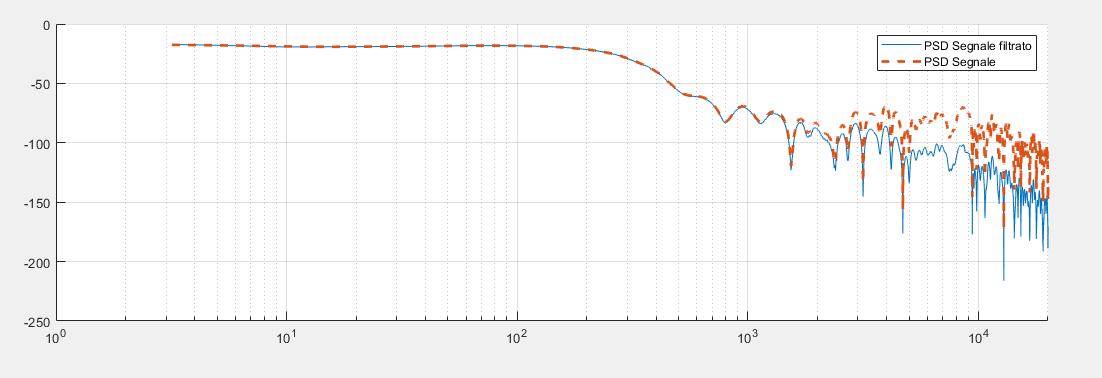
\includegraphics[width=14cm]{Effettofiltraggio}
	\caption{Effetto del filtraggio sulla PSD sel segnale della forza. Differenze evidenti si riscontrano esclusivamente ad alta frequenza.}
	\label{fig:Effettofiltraggio}
 \end{figure}

\subsection{Finestratura}

\begin{figure}
	\centering
	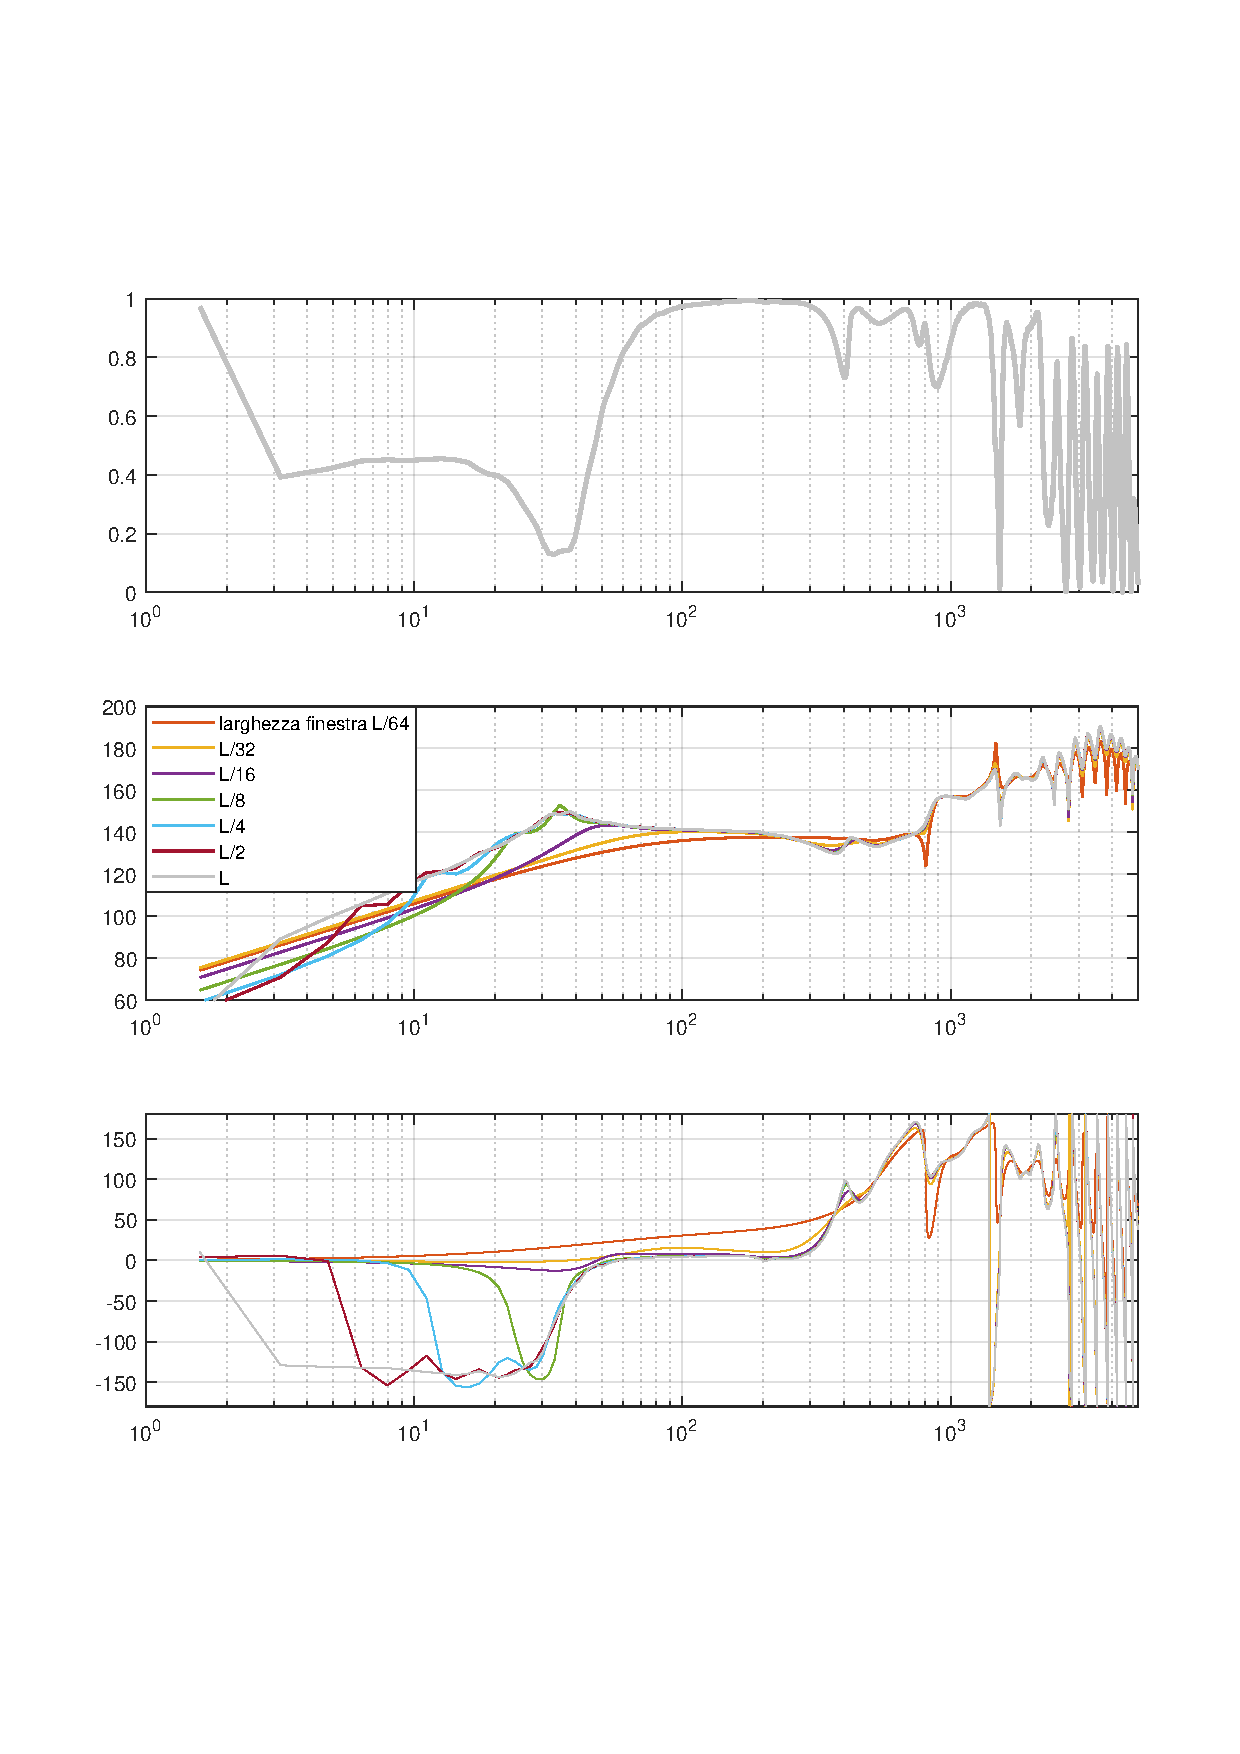
\includegraphics[width=16cm]{effettofinestra}
	\caption{Effetto della finestratura su coerenza dei segnali e modulo e fase della Dynamic Stiffness K. In alto la coerenza tra i segnali, al centro il modulo della costante elastica dinamica K e in basso la sua fase.}
	\label{fig:effettofinestra}
\end{figure}

La finestratura del segnale ha lo scopo di scongiurare l'incorrere di artefatti nella trasformata del segnale dovuti alla durata finita del segnale nel tempo. A tal fine sono state prese in esame diverse tipologie di finestre tra cui Hamming, Hann, rettangolare e se ne sono studiate le prestazioni in funzione della lunghezza delle stesse. In \figurename~\ref{fig:effettofinestra} possiamo osservare l'effetto prodotto da finestre Hann progressivamente pi\'u larghe (la 1/64 della lunghezza del campione alla lunghezza del compione). Come possiamo osservare, nessun effetto \'e riscontrabile sulla coerenz, che resta invariata al cambiare della larghezza della finestra ma lo stesso non lo si pu\'o dire per fase e modulo della Costante elastica dinamica. Allargando la finestra sopraggiungono una serie di risonanze iniziamlente non riscontrate dunque ci chiediamo se queste siano presenti nel segnale originale o piuttosto figlie della finestratura.
\subsection{Calcolo delle PSD}












 
 \end{document}